\documentclass{beamer}
%%% ========== Package setup ==========
\usepackage{xeCJK}      % Chinese words package
\usepackage{fontspec}   % Word fonts package
\usepackage{listings}
\usepackage{wrapfig}
\usepackage{multicol}   % Multicolumn package

%%% ========== Slide setting ==========
%% Slide theme setup
\usetheme{Madrid}

%% Setup chinese words encoder
\XeTeXlinebreaklocale "zh"
\XeTeXlinebreakskip = 0pt plus 1pt

%% More word fonts
% \setmainfont{Times New Roman}
\renewcommand{\familydefault}{\rmdefault}
\setCJKmainfont{標楷體}

% Setting for figure and table numbering
\setbeamertemplate{caption}[numbered]

%%% ========== Title setup ==========
\date{January 03, 2022}
\title{Meeting}
\author{Po-Hsun Wu}

%%% ========== Document ==========
\begin{document}
    \frame{\titlepage}

    \section{Progress report}

    \begin{frame}
        \frametitle{\secname}
        \begin{itemize}
            \item Study how the simulation work in Gazebo and Xplane.
        \end{itemize}
    \end{frame}

    \section{Gazebo}

    \begin{frame}
        \frametitle{\secname}
        \centering
        \begin{figure}[h!]
            \begin{multicols}{2}
                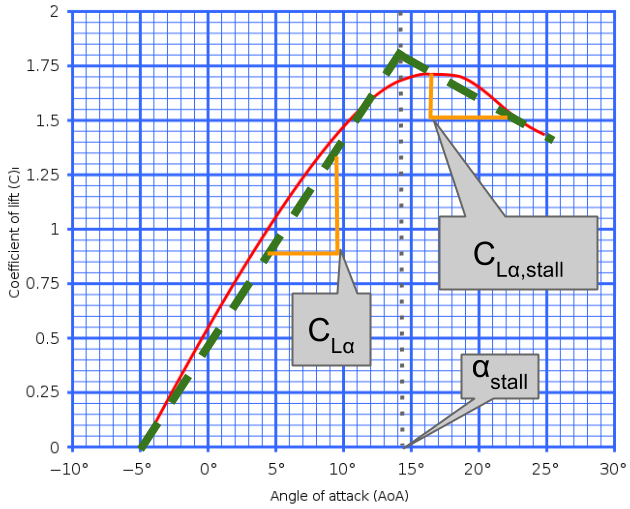
\includegraphics[width=2in]{Figs/lift_curve_simplified.png}
                \caption{Simplified lift curve}
                \columnbreak

                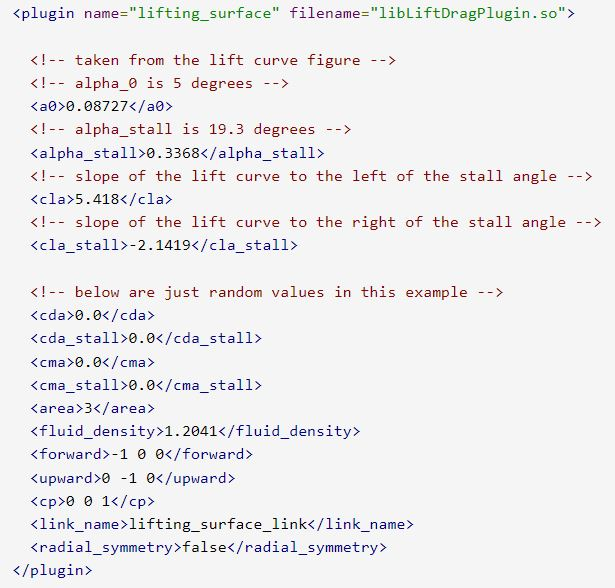
\includegraphics[width=2in]{Figs/Lift_curve_setup.JPG}
                \caption{All setup of aerodynamic object}
            \end{multicols}
        \end{figure}
    \end{frame}

    \section{Xplane}

    \begin{frame}
        \frametitle{\secname}
        \begin{multicols}{2}
            \begin{itemize}
                \item[1.] Simulation method is base on blade element theory.
                \item[2.] Find out the velocity vector of each element.
                \item[3.] Sum up all the force, and figure out the linear and angular accelerations.
            \end{itemize}
            \columnbreak

            \begin{figure}
                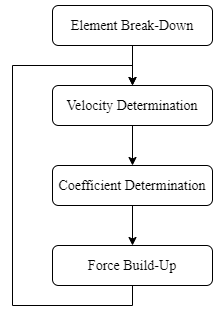
\includegraphics[scale=.3]{Figs/Xplane_simulate_flow_diagram.png}
                \caption{Flow diagram}
            \end{figure}
        \end{multicols}

    \end{frame}

\end{document}
